\subsection{Instance Reduction Analysis}
\label{subsubsec:discussion-reduction}

This section examines the impact of three reduction techniques—GCNN, ENNTH, and Drop3—on the performance, training time, testing time, and storage requirements of both the KNN and SVM algorithms.

\subsubsection{KNN Results}
In our analysis of the Hepatitis dataset, we observed that applying reduction techniques
for K-Nearest Neighbors (KNN) resulted in F1 scores similar to those obtained without any reduction.
However, the Drop3 method saw a slight decrease in mean F1 score from 0.948 to 0.864. 

In terms of training time, all reduction approaches exhibited a consistent similar duration compared to not applying reduction.

Regarding storage efficiency, the ENNTH method did not yield any reductions, while both GCNN and Drop3 achieved approximately
27\% and 20\% reductions in storage, respectively. We hypothesize that ENNTH, which focuses on removing noisy instances, did not
find any significant noise in the Hepatitis dataset, which is relatively clean.

For the Hepatitis dataset, the F1 score remained at 1.0 across all methods. Notably, only GCNN succeeded in reducing storage,
whereas ENNTH and Drop3 did not provide any reductions. This is likely because Drop3 not only removes noisy instances but also
attempts to eliminate duplicates. Its effectiveness in reducing storage for Hepatitis, but not for the Mushroom dataset, suggests
that there are fewer duplicates present in the Mushroom dataset. Similarly, ENNTH likely failed to achieve any reductions due to the lack of noise in the data.

In contrast, GCNN demonstrated a substantial 50\% reduction in storage, with a one-third decrease in training time and a halving of testing time. It is crucial to note that GCNN employs an incremental approach, unlike ENNTH and Drop3, which are decremental methods aimed at removing non-beneficial instances. This incremental approach appears to be more effective in this context.

\begin{figure}
    \centering
    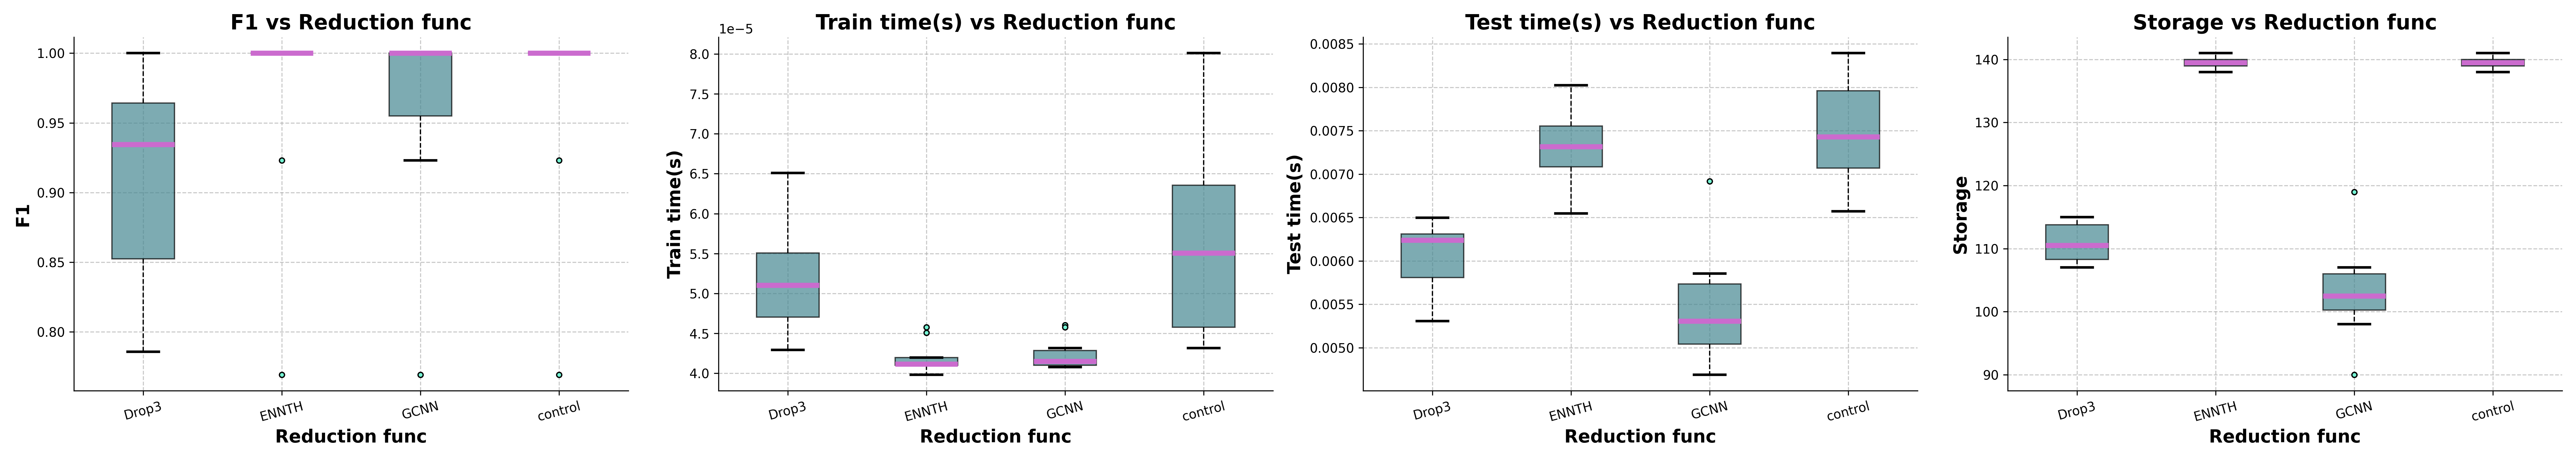
\includegraphics[width=\textwidth]{figures/KNN_reduction_effects_hepatitis.png}
    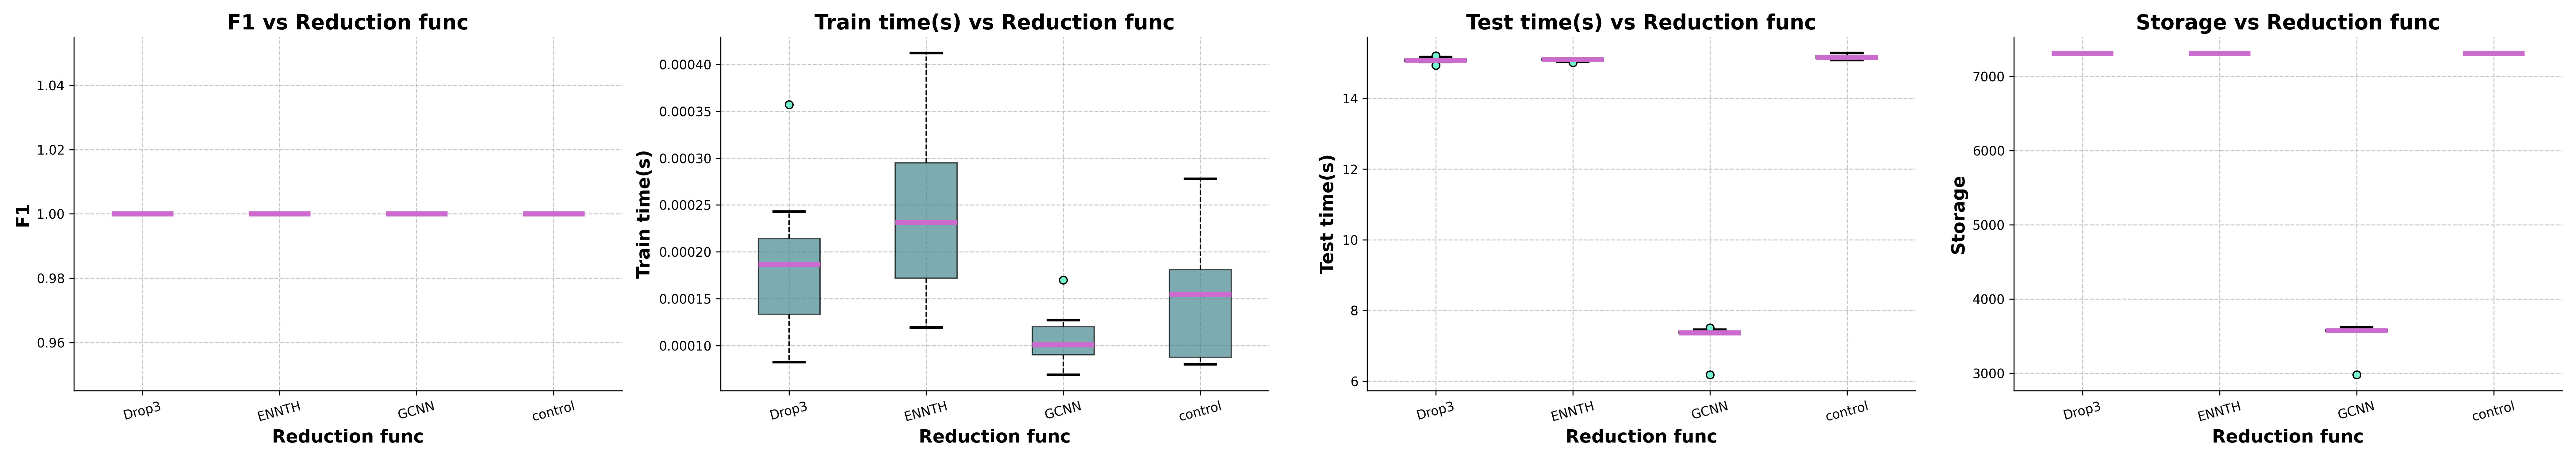
\includegraphics[width=\textwidth]{figures/KNN_reduction_effects_mushroom.png}
    \caption{Effects of reduction techniques on KNN models for the Hepatitis and Mushroom datasets respectively}
    \label{fig:KNN-reduction-effects}
\end{figure}

\subsubsection{SVM Results}

\paragraph{Hepatitis Dataset} Similarly, applying the SVM model to the reduced Hepatitis dataset yielded comparable results in terms of F1 scores,
with all accuracies remaining similar; however, the Drop3 method did result in a slight decline in accuracy.

Additionally, the training and testing times were largely consistent with those observed when no reduction was applied,
which can be attributed to the relatively small size of the dataset.

\paragraph{Mushroom Dataset} In contrast, the larger Mushroom dataset demonstrated different outcomes.
Here, GCNN significantly reduced both training and testing times. 
Specifically, while using KNN with GCNN reduction achieved a one-third reduction in training time,\\
SVM with GCNN reduction realized an impressive approximate 70\% decrease. 

For testing times, KNN with GCNN reduction saw a 50\% reduction, whereas in the case of SVM with GCNN reduction, the reduction was closer to one-third.

\begin{figure}
    \centering
    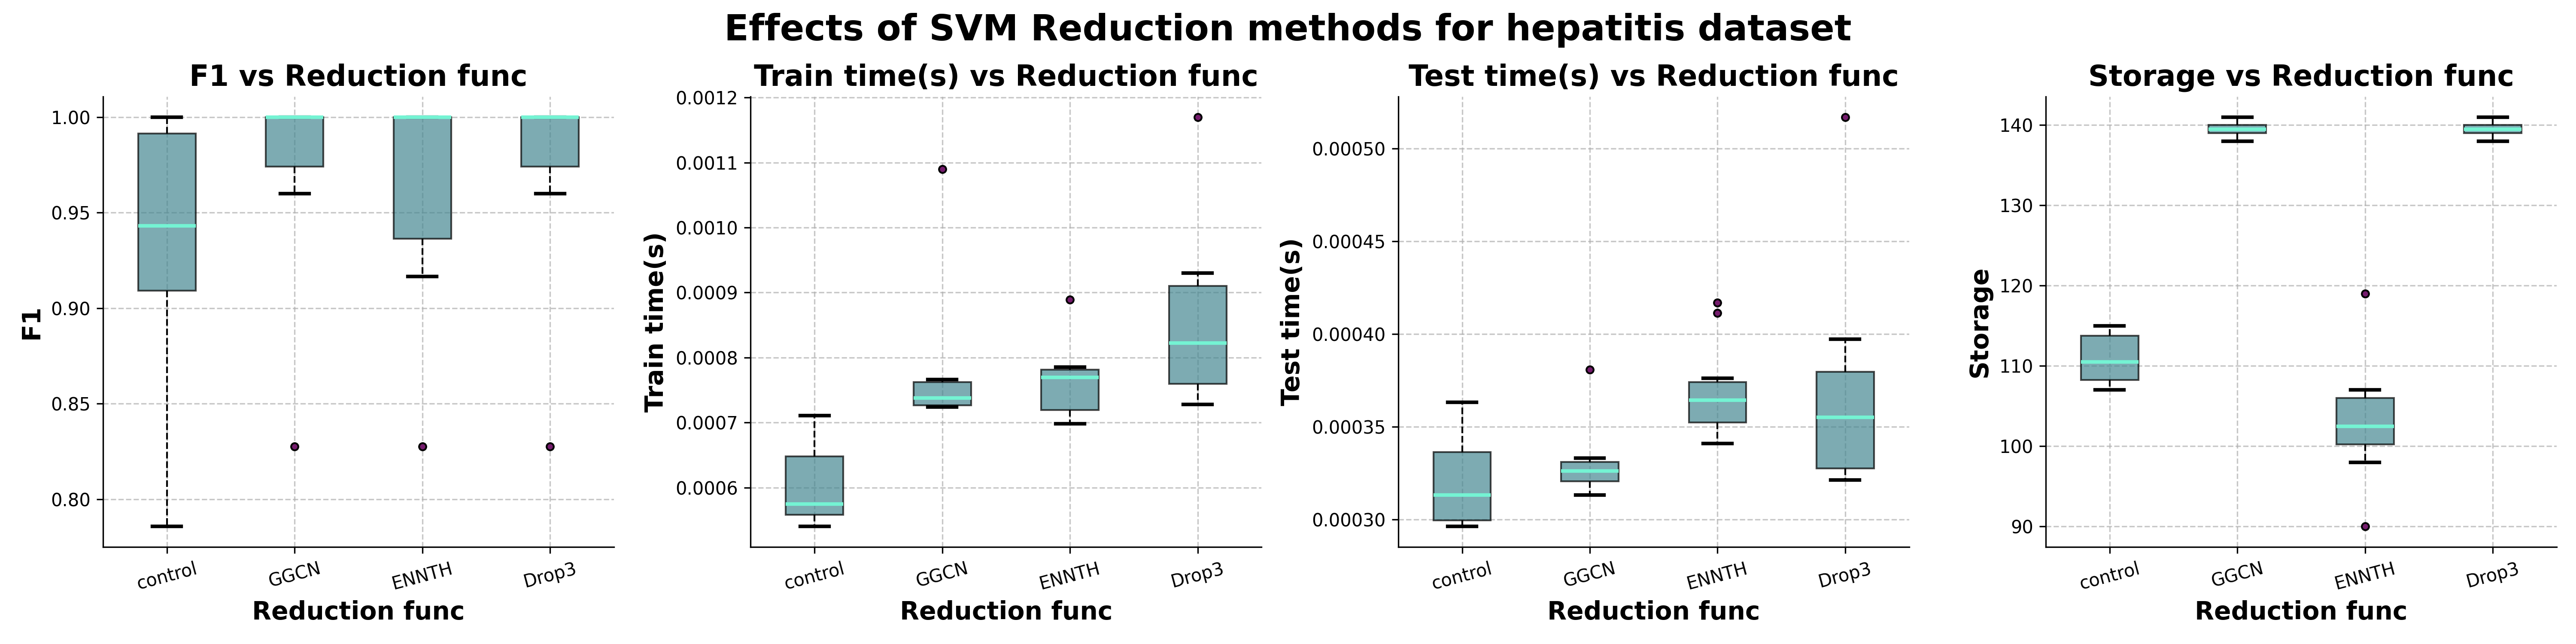
\includegraphics[width=\textwidth]{figures/SVM_reduction_effects_hepatitis.png}
    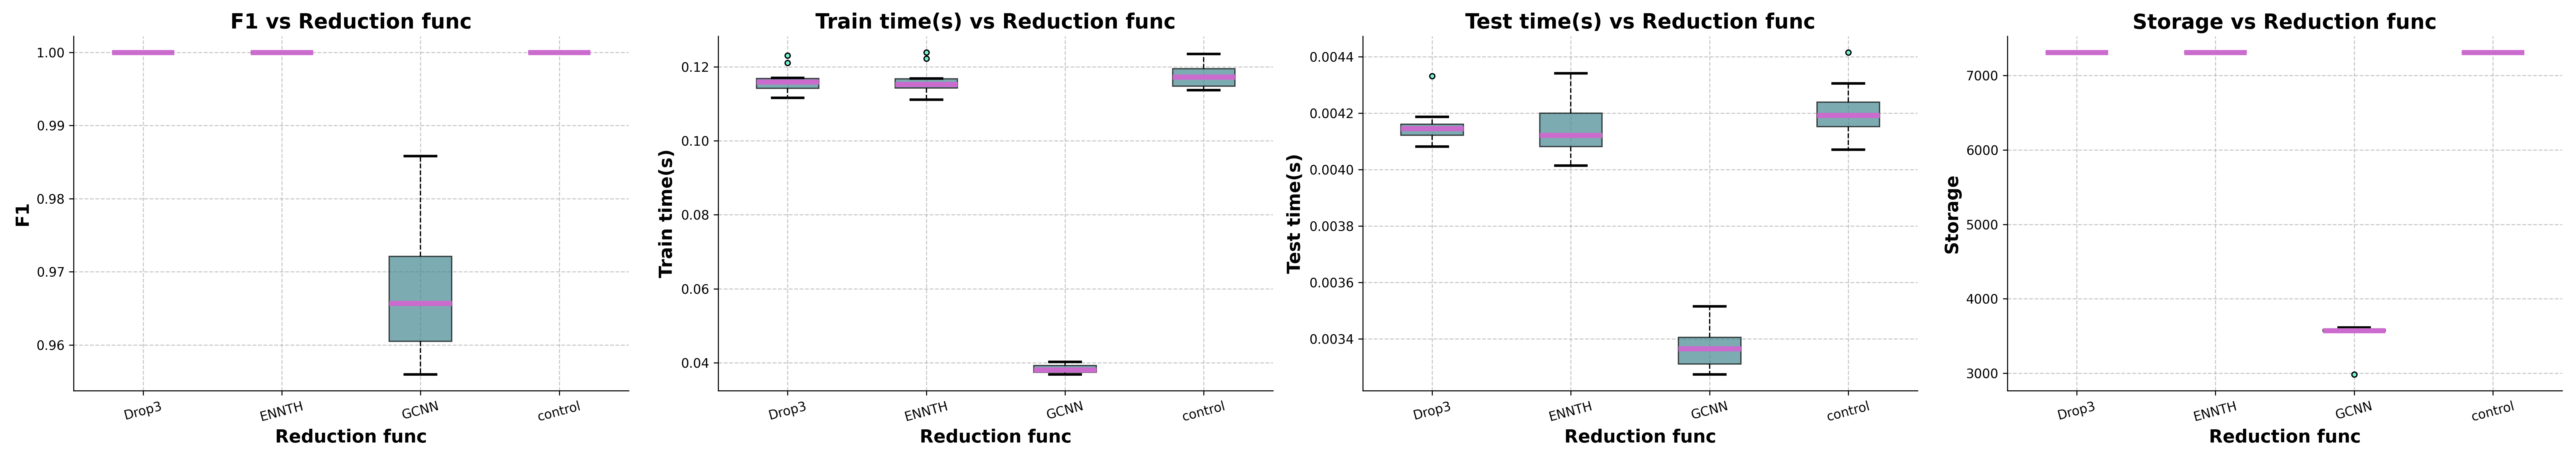
\includegraphics[width=\textwidth]{figures/SVM_reduction_effects_mushroom.png}
    \caption{Effects of reduction techniques on SVM models for the Hepatitis and Mushroom datasets respectively}
    \label{fig:SVM-reduction-effects}
\end{figure}

\begin{figure}
    \centering
    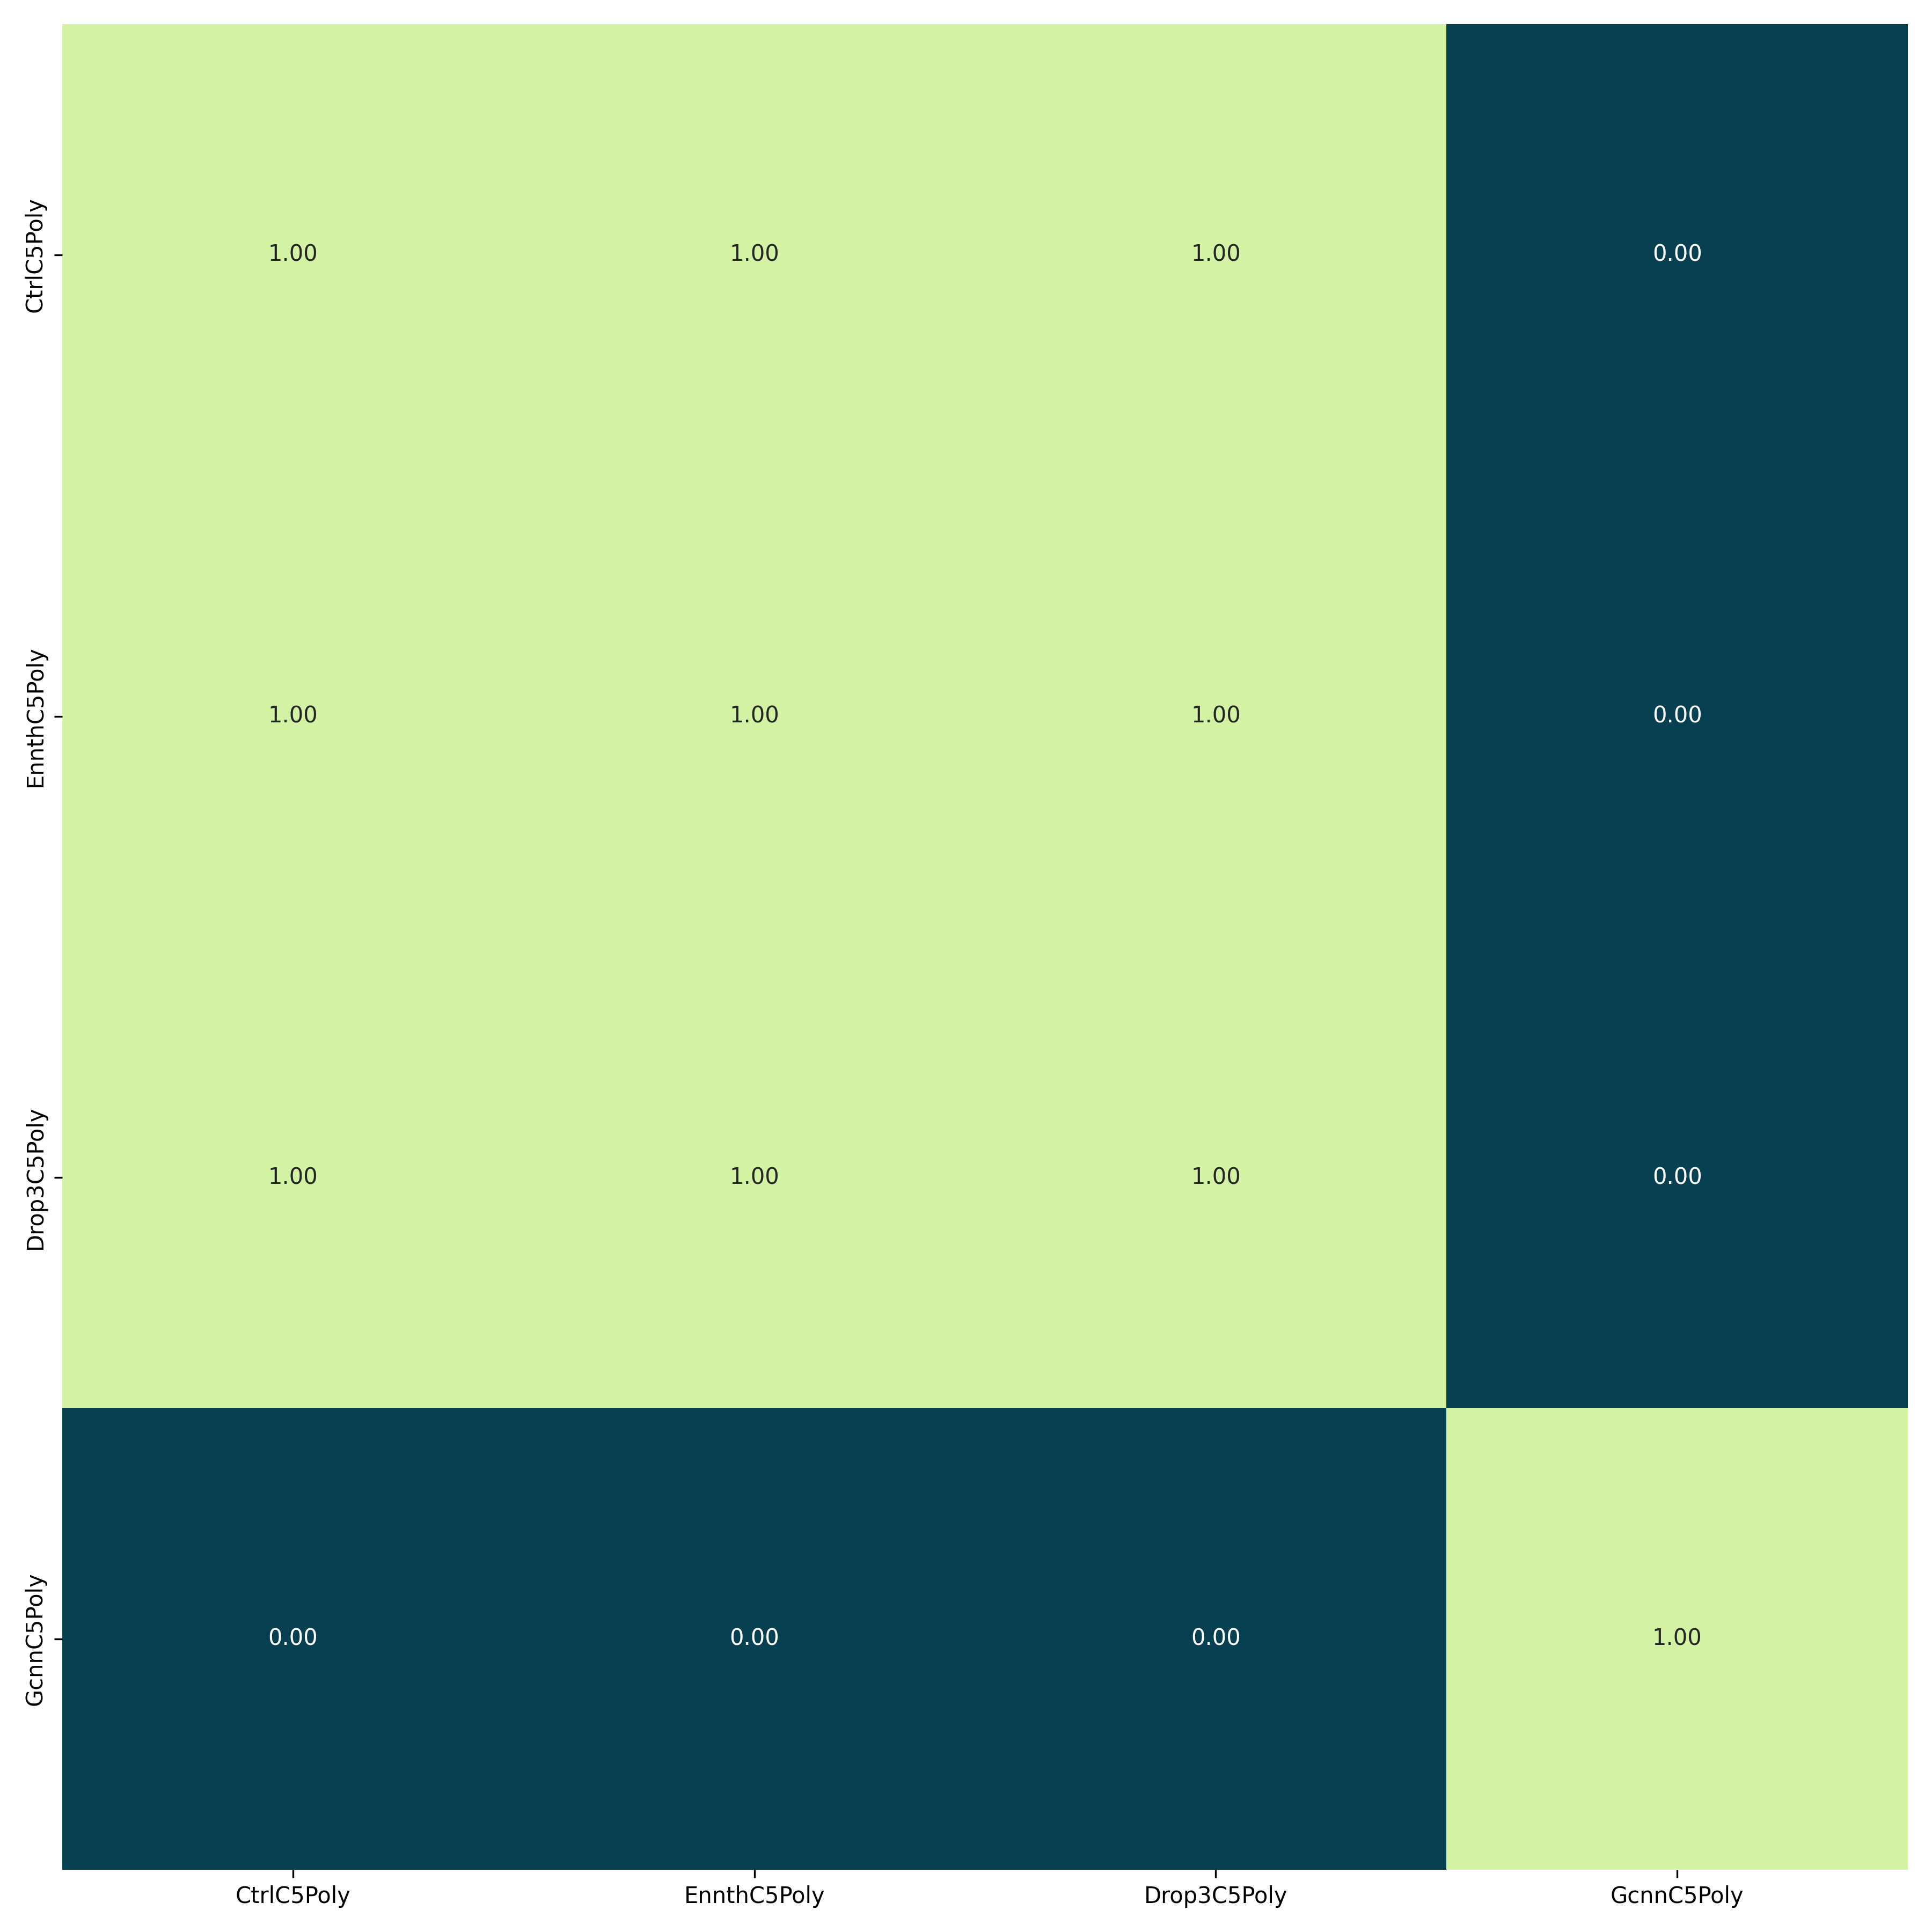
\includegraphics[width=0.5\textwidth]{figures/nemenyi_test_results_SVM_Reduction_mushroom.png}
    \caption{Nemenyi test results for SVM-Reduction models for the Mushroom dataset}
    \label{fig:nemenyi-svm-reduction-mushroom}
\end{figure}

\begin{table}
\centering
\caption{Significant Differences in SVM-Reduction Models for Mushroom}
\label{tab:svm_reduction_significant_pairs_mushroom}
\begin{tabular}{rlr}
\toprule
C & Kernel Type & Mean F1 \\
\midrule
5 & poly & 1.000 \\
5 & poly & 0.972 \\
5 & poly & 1.000 \\
5 & poly & 1.000 \\
\bottomrule
\end{tabular}
\end{table}



\paragraph{Friedman and Nemenyi Tests} Given that the Friedman test showed statistical significance for the hepatitis dataset \autoref{tab:friedman_test_results_hepatitis}, we conducted the Nemenyi post-hoc test to identify specific significant differences between reduction methods. 
For the SVM models on the Hepatitis dataset, the test revealed significant differences between GCNN (p < 0.05) and the other methods, with GCNN performing worse in terms of F1 score (see \autoref{fig:nemenyi-svm-reduction-mushroom}).
This is loss in performance may be worth the gains in training time in certain cases.

